% !Mode:: "TeX:UTF-8"

\chapter{系统实现技术方法研究}
信息管理系统的实现技术多种多样,所以选择合理的技术来实现系统也是一个重大的环节,如果所选择的技术不当,将对系统的实现造成一定的麻烦,可能还会影响系统的性能。J2EE[7]是实现信息管理系统的一种有效技术,当前用J2EE实现B/S结构的信息管理系统非常的流行且技术也越来越趋于成熟,性能也得到了非常大的提升。轻量级的J2EE应用对于小中型项目的开发带来了许多便利之处,对比于经典J2EE的简化,在保留经典J2EE应用的框架、良好的可扩展性、可维护性的基础上,简化了J2EE应用的开发,降低了J2EE应用的部署成本,基本实现过程简明了。轻量级J2EE应用面向的是用户,是一种更实际的信息化平台架构。

基于Web的J2EE Framework在J2EE的世界内已是空前繁荣,几乎每隔一两个星期就会有新的MVC框架发布。目前比较好的框架中有老牌的Struts、WebWork;新兴的有Spring MVC[9]、Tapestry、JSF等。这些大多是著名团队的作品,另外还有一些边缘团队的作品,也相当出色,如Dinamica、VRaptor等。这些框架都提供了较好的层次分隔能力。在实现良好的MVC分隔的基础上,通过提供一些现成的辅助类库,同时也促进了生产效率的提高。而如何选择一个好的框架应用在项目中,将会对项目的效率与可重用生成重大影响。

实现轻量级J2EE的Spring、Hibernate框架是在各种流行框架之中脱颖而出,逐渐成为软件开发人才,特别是WEB程序开发人才喜爱的开发技术。

本系统的开发拟采用Spring(Spring MVC)、Hibernate框架。以下是框架的简单特征与其在系统开发中的作用。

\section{Spring框架}
服务层的著名开发框架Spring[16]本身就是基于MVC结构的,此外它还具有一些良好的特性,如IOC(或DI)和AOP。Inversion of Control(IOC) 控制反转,就是程序的主控权由应用程序代码本身转移到了框架或容器。Dependency Injection(DI)依赖注入,是一个更能描述其特点的名字,可以解释为容器在运行期将某种依赖关系注入到组件中。

Aspect-Oriented Programming(AOP)面向方面编程通过提供另一种考虑程序结构的方式来补充面向对象编程(OOP)。面向对象将应用程序分解成各个层次的对象,而AOP将程序分解成各个方面或者说关注点。这种方式能够模块化例如事务管理这种横切多个对象的关注点(这种关注点术语称作横切关注点)。AOP框架是Spring的一个关键组件,但Spring IOC容器(Bean Factory)和(Application Context)并不依赖于AOP ,这就意味着如果不需要使用AOP则可不用。AOP补充了Spring IOC ,以提供一个有效的中间件解决方案。[21]

Spring的精简项目的代码量方面做出了非常出色的工作,将大量需要重复书写的代码提取出来,进行切面编程。配置文件的灵活性也使项目的灵活性得到的加强,可以在不改变代码的情况下,而只有改变其中的配置文件实现整个系统的改变。

\section{Spring框架的MVC实现[17]——Spring MVC}
Spring的WEB框架是围绕DispatcherServlet来进行设计的。DispatcherServlet的作用是将请求分发到不同的处理器。图~\ref{fig:req_proc}~展示了DispatcherServlet对请求的处理流程。
\begin{figure}[htbp]
\centering
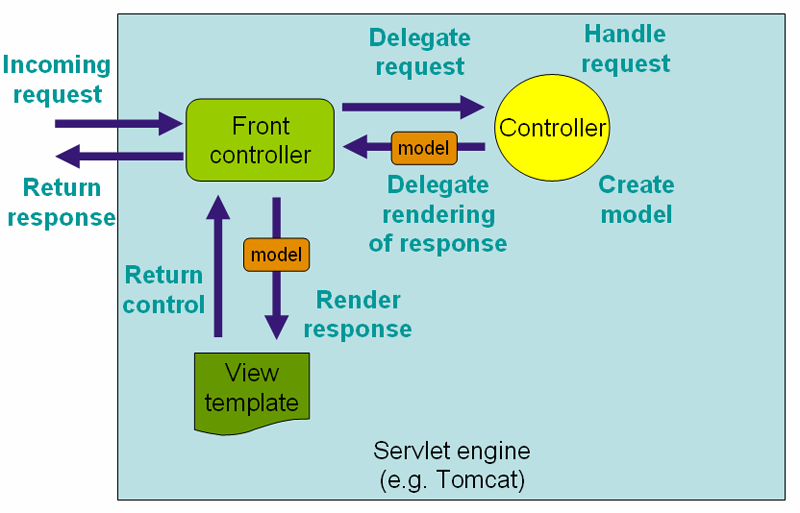
\includegraphics[width=11.65cm]{req_proc}
\caption{Spring Web MVC处理请求工作流程}\label{fig:req_proc}
\vspace{\baselineskip}
\end{figure}
\begin{table}[htbp]
\caption{WebApplicationContext中特殊的bean}\label{tab:bean}
\vspace{0.5em}\centering\wuhao
\begin{tabular}{|m{6cm}|m{6cm}|}
\toprule[1.5pt]
名称 & 描述\\
\midrule[1pt]
控制器(Controller) & 控制器实现的是MVC中Controller那部分\\ \hline
处理器映射(Handler mapping) & 处理器映射包含预处理器(pre-processor),后处理器(post-processor)和控制器的列表,它们在符合某种条件时才被执行(例如符合控制器指定的URL)\\ \hline
视图解析器(View resolvers) & 视图解析器 可以将视图名解析为对应的视图\\ \hline
本地化解析器(Locale resolver) & 本地化解析器能够解析用户正在使用的本地化配置,以提供国际化视图\\ \hline
主题解析器(Theme resolver) & 主题解析器能够解析你的web应用所使用的主题,以提供个性化的布局\\ \hline
上传文件解析器(multipart file resolver) & 上传文件解析器提供HTML表彰文件上传功能\\ \hline
处理异常解析器(Handler exception resolver(s)) & 处理器异常解析器可以将异常对应到视图,或者实现更加复杂的异常处理代码\\
\bottomrule[1.5pt]
\end{tabular}
\vspace{\baselineskip}
\end{table}
DispatcherServlet实际上是一个Servlet,它从HttpServlet继承而来。和其它Servlet一样,DispatcherServlet定义在web应用的web.xml文件中。Spring的Dispatcher有一组特殊的bean,如表~\ref{tab:bean}~所示,用来处理请求和渲染相应的视图。

\section{Hibernate框架}
Hibernate[18]是一种Java语言下的对象关系映射解决方案,它是一种自由、开源的软件。它用来把对象模型表示的对象映射到基于SQL的关系模型结构中去,为面向对象的领域模型到传统的关系型数据库的映射,提供了一个使用方便的框架。Hibernate不仅管理Java类到数据库表的映射(包括从Java数据类型到SQL数据类型的映射),还提供数据查询和获取数据的方法,可以大幅度减少开发时人工使用SQL和JDBC处理数据的时间。它的设计目标是将软件开发人员从大量相同的数据持久层相关编程工作中解放出来。无论是从设计草案还是从一个遗留数据库开始,开发人员都可以采用Hibernate。

下面从Hibernate的体系结构与Hibernate API两方面对Hibernate进行介绍。

(1) hibernate体系结构简介
\begin{figure}[htbp]
\centering
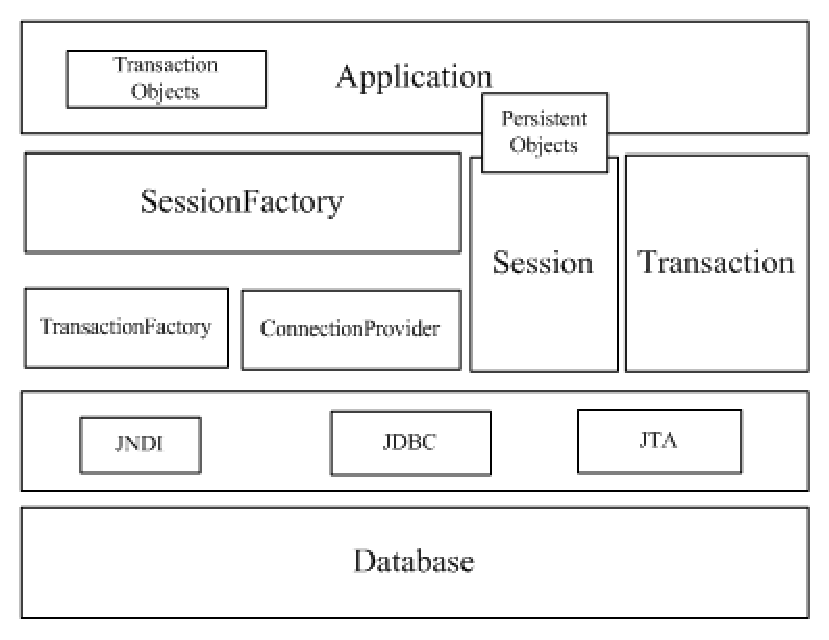
\includegraphics[width=10.01cm]{arch}
\caption{Hibernate体系结构图}\label{fig:arch}
\vspace{\baselineskip}
\end{figure}
图~\ref{fig:arch}~各对象的说明如下:\par
SessionFactory:针对单个数据库映射关系经过编译后的内在镜像,是线程安全的,它是生成Session的工厂。\par
Session:表示应用程序与持久存储层之间交互操作的一个单纯种对象,此对象生存期很短。其隐藏了JDBC连接,也是Transaction的工厂。\par
持久对象及集合:带有持久化状态的、具有业务功能的单线程对象,此对象生存期很短。这些对象可能是普通的JavaBeans/POJO,唯一特殊的是他们正与(仅仅一个)Session相关联。一旦这个Session被关闭,这些对象就会脱离持久化状态,这样就可被应用程序的任何层自由使用。\par
瞬态(transient)和脱管(detached)的对象及其集合:那些目前没有与session关联的持久化类实例。他们可能是在被应用程序实例化后,尚未进行持久化的对象,也可能是因为实例化他们的Session已经被关闭而脱离持久化的对象。\par
事务Transaction:应用程序用来指定原子操作单元范围的对象,它是单线程了,生命周期很短。\par
Hibernate作为模型/数据访问层。它通过配置文件(hiberante.cfg.xml或hibernate.properties和映射文件(*.hbm.xml)把java对象或持久化对象(Persistent Obeject,PO)映射到数据库中的数据表,然后通过操作PO,对数据库中的表进行各种操作。

(2) Hibernate API简介\par
Hibernate API中的接口可分为以下几类:\par
(a)	提供访问数据库的操作的接口,包括Session、Transaction、Query接口。\par
(b)	用于配置Hibernate的接口,Configuration(如下在Spring应用中,将由Spring来完成Hibernate的相关配置)。\par
(c)	间接接口,使应用程序接受Hibernate内部发生的事件,并作出相应的回应,包括:Interceptor、LifeCycle、Validatable。\par
(d)	用户于扩展Hibernate功能的接口,如UserType、CompositeUserType接口。\par
Hibernate内部还封装了JDBC、JTA(Java Transaction API)和JNDI(Java Naming And Directory Interface)。其中,JDBC提供底层的数据访问操作,只要用户提供了相应的JDBC驱动程序,Hibernate可以访问任何一个数据库系统。JTA和JNDI使Hibernate能够和J2EE应用服务器集成。具体接口间的协作如图~\ref{fig:interface}~所示。 
\begin{figure}[htbp]
\centering
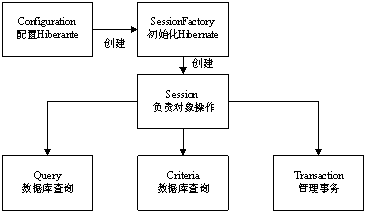
\includegraphics[width=11.1cm]{interface}
\caption{Hibernate核心接口}\label{fig:interface}
\vspace{\baselineskip}
\end{figure}

\section{AJAX技术}
AJAX[21]全称为“Asynchronous JavaScript and XML”(异步JavaScript和XML),是指一种创建交互式网页应用的网页开发技术。主要包含了以下几点技术:基于web标准(standards-based presentation)XHTML+CSS的表示;使用DOM(Document Object Model)进行动态显示及交互;使用XML和XSLT进行数据交换及相关操作;使用XMLHttpRequest进行异步数据查询、检索;使用JavaScript[22]将所有的东西绑定在一起。类似于DHTML或LAMP,AJAX不是指一种单一的技术,而是有机地利用了一系列相关的技术。使用Ajax的最大优点,就是能在不更新整个页面的前提下维护数据,这使得Web应用程序更为迅捷地回应用户动作,并避免了在网络上发送那些没有改变过的信息[23]。

\section{框架之间的有机整合}
Spring与Hibernate的集成是通过配置完成的。通过一个个的配置文件实现两者框架之间的连接。

Hibernate与Spring的集成。Spring 为持久层的开发提供了强有力的支持,其中对于Hibernate 的支持包括HibernateTemplate , HibernateInterceptor 和Hibernate transaction manager 。Hibernate 的连接、事务管理等是由SessionFactory 开始的,SessionFactory底层的DataSource 可以使用Spring 的IOC 注入,然后将SessionFactory 注入到相应的对象中。
